\documentclass[10pt,a4paper]{article}
\usepackage[margin=0.78in]{geometry}
\usepackage[T1]{fontenc}
\usepackage{lmodern,microtype}
\usepackage{graphicx,booktabs,tabularx,array}
\usepackage[table]{xcolor}
\usepackage{caption,enumitem,hyperref,parskip}
\definecolor{DeepTeal}{HTML}{006B70}
\definecolor{SoftTeal}{HTML}{E8F4F3}
\definecolor{Slate}{HTML}{334155}
\hypersetup{colorlinks=true,linkcolor=DeepTeal,urlcolor=DeepTeal}
\captionsetup{font=small,labelfont={bf,color=DeepTeal},skip=6pt}
\setlength{\parskip}{5pt}
\setlist{nosep,leftmargin=1.3em}
\title{\vspace{-1.4cm}\color{DeepTeal}\bfseries When Do Released Labels Help?\\[3pt]
\large A Label-Safe Recalibration Replay on UCI Gas Sensor Cohorts}
\author{IDM-Viz Phase 3 --- exploratory external extension}
\date{16 November 2026}
\begin{document}\maketitle\vspace{-0.5cm}
\begin{abstract}\small
The Phase 3 external evaluation found severe batch-1 calibration-transfer failure on UCI dataset 224. This extension replays the already frozen class predictions under explicit whole-cohort label-release delays and updates only a one-dimensional correctness calibrator. Across batches 2--10 (13,465 rows), cumulative released-label logistic recalibration reduced equal-batch accuracy-estimation MAE from 0.545 for frozen calibration to 0.169, 0.227, and 0.283 at delays of 0, 1, and 2 acquisition cohorts. The improvement is descriptive for one ordered dataset sequence. Labels arrive on simulated cohort clocks, not observed timestamps; no independent-stream or population guarantee follows.
\end{abstract}
\vspace{-2mm}\noindent\colorbox{SoftTeal}{\parbox{0.97\linewidth}{\textbf{What this adds.} The forecast pipeline enforces a strict release-before-forecast rule and isolates evaluator truth. It demonstrates delayed-label behavior on the external sequence while preserving its frozen classifier and original Day 2/Day 3 evidence.}}
\section{Question and protocol}
The Day 3 report identified a major limitation: the UCI result was a retrospective cohort evaluation, not an as-of-time replay. We ask whether a fixed scalar confidence-to-correctness map updated with already released outcomes can improve subsequent cohort accuracy estimates, and how the result changes when labels are delayed.

The source archive and original batch-1 train/calibration/reference split are unchanged. The multinomial logistic classifier, its preprocessing, class predictions, and confidence values are frozen. The initial logistic correctness map is fitted on batch-1 calibration examples. The online variant refits the same one-dimensional logistic family cumulatively on those historical examples and only eligible released cohorts. For target batch $b$, source cohort $j$ is eligible at delay $d$ only if $j+d<b$. This strict inequality prevents current-cohort labels from entering its own forecast. Delays $0,1,2$ are measured in whole cohort steps; because cohort sizes differ, they are not fixed row counts or elapsed time.

Comparators are frozen calibration, raw Average Confidence, and batch-1 reference accuracy. We report equal-batch MAE and bias for cohort accuracy forecasts, row-weighted Brier score for per-row correctness probabilities, and equal-batch ECE-10. No batch-level inferential test is used: nine ordered cohorts from one source are not independent replications.

\section{Results}
\begin{figure}[ht]
\centering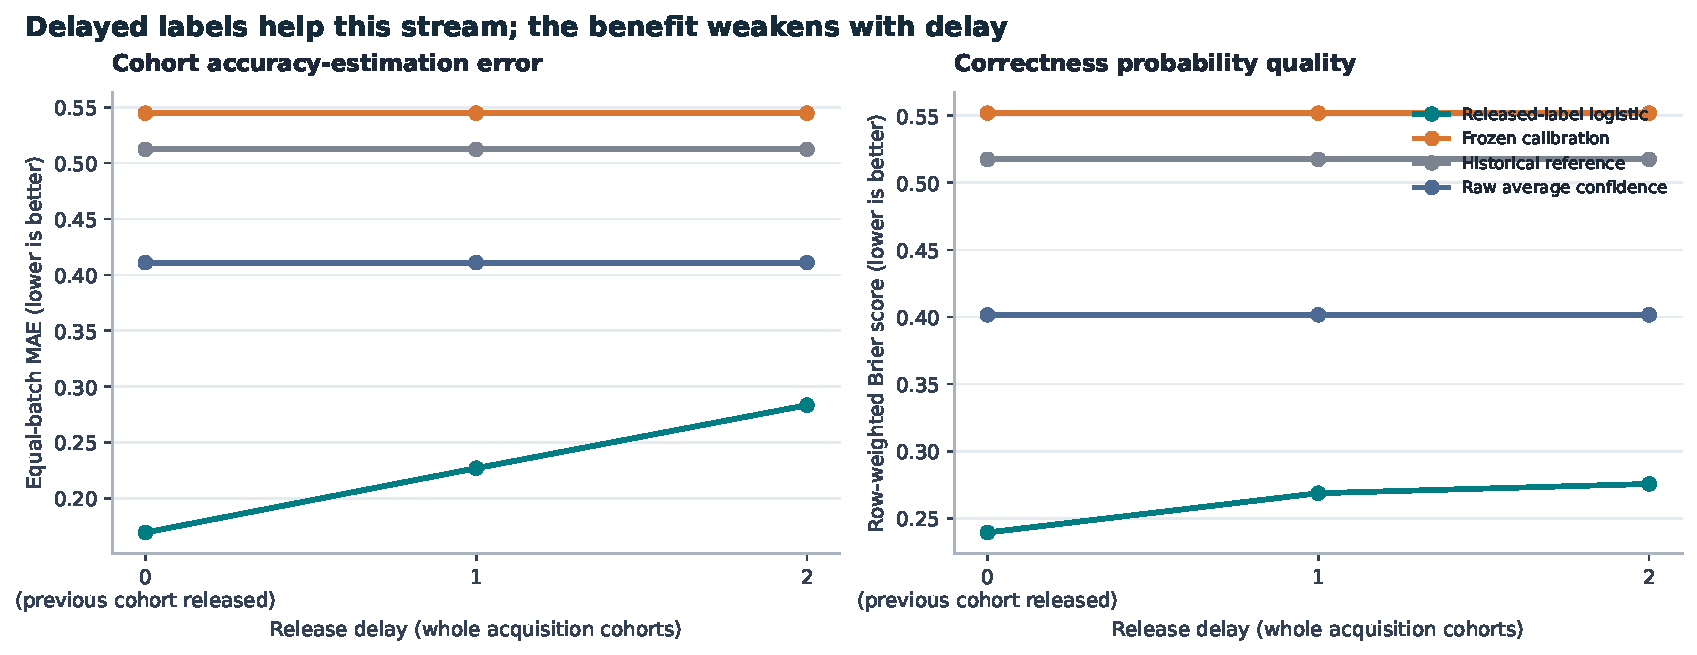
\includegraphics[width=\linewidth]{recalibration_by_delay.pdf}
\caption{Forecast error and correctness-probability score across release delays. Lower values are better. Frozen and non-updated baselines repeat across delay settings by construction.}
\end{figure}
\begin{table}[ht]
\centering\small
\caption{All metrics aggregate batches 2--10. MAE and bias weight each cohort equally; Brier weights rows; ECE-10 is averaged equally over cohorts.}
\rowcolors{2}{SoftTeal}{white}
\begin{tabular}{r l r r r r}\toprule
Delay & Method & Accuracy MAE & Bias & Brier & ECE-10\\\midrule
0 & Released-label logistic & 0.169 & 0.169 & 0.239 & 0.188 \\
0 & Frozen calibration & 0.545 & 0.545 & 0.552 & 0.545 \\
0 & Historical reference & 0.512 & 0.512 & 0.517 & 0.512 \\
0 & Raw average confidence & 0.411 & 0.411 & 0.402 & 0.412 \\
1 & Released-label logistic & 0.227 & 0.227 & 0.269 & 0.245 \\
1 & Frozen calibration & 0.545 & 0.545 & 0.552 & 0.545 \\
1 & Historical reference & 0.512 & 0.512 & 0.517 & 0.512 \\
1 & Raw average confidence & 0.411 & 0.411 & 0.402 & 0.412 \\
2 & Released-label logistic & 0.283 & 0.283 & 0.276 & 0.290 \\
2 & Frozen calibration & 0.545 & 0.545 & 0.552 & 0.545 \\
2 & Historical reference & 0.512 & 0.512 & 0.517 & 0.512 \\
2 & Raw average confidence & 0.411 & 0.411 & 0.402 & 0.412 \\
\bottomrule\end{tabular}
\end{table}

The cumulative released-label calibrator has lower error and Brier score than the frozen map in this sequence at all three delays, with weaker performance as more release delay is imposed. At delay zero, its MAE is 0.169 versus 0.545 for the frozen calibrator; at delay two it is 0.283. The raw confidence and historical-reference baselines have MAEs 0.411 and 0.512. All methods remain positively biased in the aggregate: released calibration narrows but does not remove overestimation. These are not expected out-of-sample gains beyond this sequence.

\begin{figure}[ht]
\centering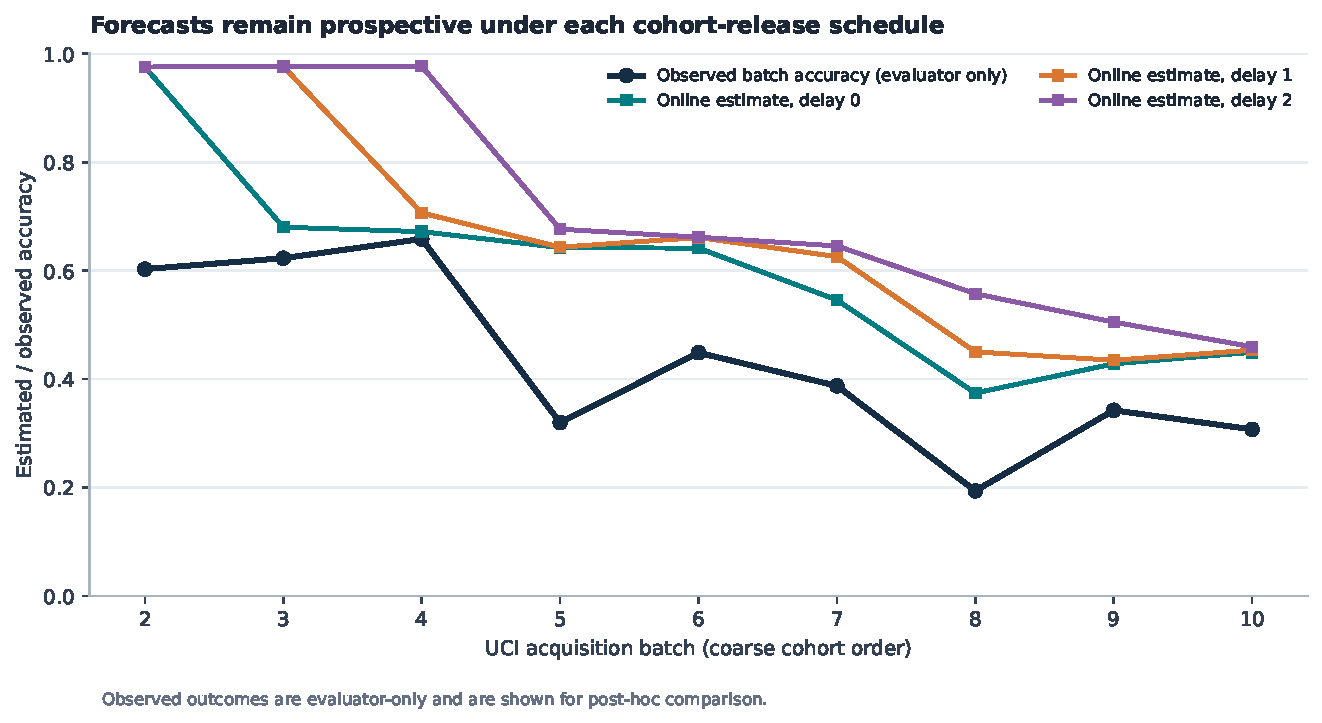
\includegraphics[width=0.9\linewidth]{cohort_accuracy_forecasts.pdf}
\caption{Per-batch accuracy forecasts made before each cohort's outcome release. Observed accuracy is shown only for evaluator comparison. Delayed methods use less recent correctness evidence.}
\end{figure}

\section{External metadata correction}
The original external runner reported the full batch-1 class counts alongside the 89-row reference evaluation denominator. A new versioned run now separates source-cohort composition (445 rows) from the evaluated reference partition (89 rows), with each count/proportion pair using its own named population. The corrected metadata sums to one in both populations. Re-running the classifier pipeline reproduced the original cohort accuracy, macro-F1, calibrated estimates, intervals, and input alarm counts exactly; only the explicitly clarified population metadata changed.

\section{Limitations and conclusion}
This replay resolves a code/evidence gap, not the underlying external calibration-transfer weakness. It uses one dataset in acquisition order, with coarse batch identifiers and synthetic release clocks; actual label-arrival times are unknown. The analysis is outcome-informed because the prior external failure motivated it. Cohort sizes are highly unequal, only nine future cohorts are evaluated, and no confidence interval is warranted as though batches were independent. The adaptive calibration curve is fit on the same ordered sequence being diagnosed, so the numbers describe this prequential replay rather than a separately held-out stream. There is no causal attribution, certified accuracy bound, natural-domain generalization, or human-benefit evaluation.

The result provides a reproducible example of the intended delayed-label mechanism and a useful negative boundary: delayed correctness feedback can reduce estimation error on this stream, yet estimates remain biased and delay degrades performance. It does not make unlabeled confidence or the plug-in interval safe under arbitrary conditional shift.

\section*{Reproduction and provenance}
From the repository root, with the configured Anaconda environment:
\begin{verbatim}
$python = 'C:/Users/hp/anaconda3/python.exe'
& $python -m pytest tests/phase3/test_uci224_delayed_replay.py tests/phase3/test_uci224_metadata_semantics.py -q
& $python scripts/evaluate_uci224_day2.py --out results/phase3/external_uci224_day2_metadata_NEW
& $python scripts/run_uci224_delayed_replay.py --source-run results/phase3/external_uci224_day2_v2 --out results/phase3/uci224_delayed_replay_NEW
& $python scripts/evaluate_uci224_delayed_replay.py --run results/phase3/uci224_delayed_replay_NEW
\end{verbatim}
The protocol, source hashes, release audit, label-free forecast arrays, isolated evaluator truth, per-cohort metrics, summary, and figures accompany this report. The submitted Phase 2 DOCX is unchanged and remains the methodological basis. No instructor feedback or human study is claimed.
\end{document}
